% Options for packages loaded elsewhere
\PassOptionsToPackage{unicode}{hyperref}
\PassOptionsToPackage{hyphens}{url}
\PassOptionsToPackage{dvipsnames,svgnames,x11names}{xcolor}
%
\documentclass[
  12pt,
  letterpaper,
  egregdoesnotlikesansseriftitles]{scrreprt}

\usepackage{amsmath,amssymb}
\usepackage{iftex}
\ifPDFTeX
  \usepackage[T1]{fontenc}
  \usepackage[utf8]{inputenc}
  \usepackage{textcomp} % provide euro and other symbols
\else % if luatex or xetex
  \usepackage{unicode-math}
  \defaultfontfeatures{Scale=MatchLowercase}
  \defaultfontfeatures[\rmfamily]{Ligatures=TeX,Scale=1}
\fi
\usepackage{lmodern}
\ifPDFTeX\else  
    % xetex/luatex font selection
  \setmainfont[]{Palatino Linotype}
\fi
% Use upquote if available, for straight quotes in verbatim environments
\IfFileExists{upquote.sty}{\usepackage{upquote}}{}
\IfFileExists{microtype.sty}{% use microtype if available
  \usepackage[]{microtype}
  \UseMicrotypeSet[protrusion]{basicmath} % disable protrusion for tt fonts
}{}
\makeatletter
\@ifundefined{KOMAClassName}{% if non-KOMA class
  \IfFileExists{parskip.sty}{%
    \usepackage{parskip}
  }{% else
    \setlength{\parindent}{0pt}
    \setlength{\parskip}{6pt plus 2pt minus 1pt}}
}{% if KOMA class
  \KOMAoptions{parskip=half}}
\makeatother
\usepackage{xcolor}
\setlength{\emergencystretch}{3em} % prevent overfull lines
\setcounter{secnumdepth}{5}
% Make \paragraph and \subparagraph free-standing
\ifx\paragraph\undefined\else
  \let\oldparagraph\paragraph
  \renewcommand{\paragraph}[1]{\oldparagraph{#1}\mbox{}}
\fi
\ifx\subparagraph\undefined\else
  \let\oldsubparagraph\subparagraph
  \renewcommand{\subparagraph}[1]{\oldsubparagraph{#1}\mbox{}}
\fi


\providecommand{\tightlist}{%
  \setlength{\itemsep}{0pt}\setlength{\parskip}{0pt}}\usepackage{longtable,booktabs,array}
\usepackage{calc} % for calculating minipage widths
% Correct order of tables after \paragraph or \subparagraph
\usepackage{etoolbox}
\makeatletter
\patchcmd\longtable{\par}{\if@noskipsec\mbox{}\fi\par}{}{}
\makeatother
% Allow footnotes in longtable head/foot
\IfFileExists{footnotehyper.sty}{\usepackage{footnotehyper}}{\usepackage{footnote}}
\makesavenoteenv{longtable}
\usepackage{graphicx}
\makeatletter
\def\maxwidth{\ifdim\Gin@nat@width>\linewidth\linewidth\else\Gin@nat@width\fi}
\def\maxheight{\ifdim\Gin@nat@height>\textheight\textheight\else\Gin@nat@height\fi}
\makeatother
% Scale images if necessary, so that they will not overflow the page
% margins by default, and it is still possible to overwrite the defaults
% using explicit options in \includegraphics[width, height, ...]{}
\setkeys{Gin}{width=\maxwidth,height=\maxheight,keepaspectratio}
% Set default figure placement to htbp
\makeatletter
\def\fps@figure{htbp}
\makeatother
\newlength{\cslhangindent}
\setlength{\cslhangindent}{1.5em}
\newlength{\csllabelwidth}
\setlength{\csllabelwidth}{3em}
\newlength{\cslentryspacingunit} % times entry-spacing
\setlength{\cslentryspacingunit}{\parskip}
\newenvironment{CSLReferences}[2] % #1 hanging-ident, #2 entry spacing
 {% don't indent paragraphs
  \setlength{\parindent}{0pt}
  % turn on hanging indent if param 1 is 1
  \ifodd #1
  \let\oldpar\par
  \def\par{\hangindent=\cslhangindent\oldpar}
  \fi
  % set entry spacing
  \setlength{\parskip}{#2\cslentryspacingunit}
 }%
 {}
\usepackage{calc}
\newcommand{\CSLBlock}[1]{#1\hfill\break}
\newcommand{\CSLLeftMargin}[1]{\parbox[t]{\csllabelwidth}{#1}}
\newcommand{\CSLRightInline}[1]{\parbox[t]{\linewidth - \csllabelwidth}{#1}\break}
\newcommand{\CSLIndent}[1]{\hspace{\cslhangindent}#1}

%%%%------------   René --------------------------------------%%%%%


%%%%%%%%%%%%%%%%%%%%%%%%%
%% Seitenstil
%%%%%%%%%%%%%%%%%%%%%%%%%

% % Seiten mit Kapitelüberschriften
% \usepackage{fancyhdr}

% \pagestyle{fancy}
% \fancyhead{} % Löscht den Standardinhalt der Kopfzeile
% \renewcommand{\headrulewidth}{0pt} % Entfernt die horizontale Linie in der Kopfzeile
% \fancyhead[L]{\leftmark} % Setzt die Seitenzahl und Kapitel/Section-Titel links in die Kopfzeile

	
% Wird für die Tabelle im Titelblatt der Experten verwendet:
%Array
\usepackage{array}
%Neue Definition für Tabelleneinträge
% linksbündig mit Breitenangabe
\newcolumntype{L}[1]{>{\raggedright\arraybackslash}p{#1}} 
% zentriert mit Breitenangabe
\newcolumntype{C}[1]{>{\centering\arraybackslash}p{#1}} 
% rechtsbündig mit Breitenangabe
\newcolumntype{R}[1]{>{\raggedleft\arraybackslash}p{#1}} 

\usepackage[a4paper, margin=3cm]{geometry}
\makeatletter
\makeatother
\makeatletter
\@ifpackageloaded{bookmark}{}{\usepackage{bookmark}}
\makeatother
\makeatletter
\@ifpackageloaded{caption}{}{\usepackage{caption}}
\AtBeginDocument{%
\ifdefined\contentsname
  \renewcommand*\contentsname{Inhaltsverzeichnis}
\else
  \newcommand\contentsname{Inhaltsverzeichnis}
\fi
\ifdefined\listfigurename
  \renewcommand*\listfigurename{Abbildungsverzeichnis}
\else
  \newcommand\listfigurename{Abbildungsverzeichnis}
\fi
\ifdefined\listtablename
  \renewcommand*\listtablename{Tabellenverzeichnis}
\else
  \newcommand\listtablename{Tabellenverzeichnis}
\fi
\ifdefined\figurename
  \renewcommand*\figurename{Abbildung}
\else
  \newcommand\figurename{Abbildung}
\fi
\ifdefined\tablename
  \renewcommand*\tablename{Tabelle}
\else
  \newcommand\tablename{Tabelle}
\fi
}
\@ifpackageloaded{float}{}{\usepackage{float}}
\floatstyle{ruled}
\@ifundefined{c@chapter}{\newfloat{codelisting}{h}{lop}}{\newfloat{codelisting}{h}{lop}[chapter]}
\floatname{codelisting}{Listing}
\newcommand*\listoflistings{\listof{codelisting}{Listingverzeichnis}}
\makeatother
\makeatletter
\@ifpackageloaded{caption}{}{\usepackage{caption}}
\@ifpackageloaded{subcaption}{}{\usepackage{subcaption}}
\makeatother
\makeatletter
\@ifpackageloaded{tcolorbox}{}{\usepackage[skins,breakable]{tcolorbox}}
\makeatother
\makeatletter
\@ifundefined{shadecolor}{\definecolor{shadecolor}{rgb}{.97, .97, .97}}
\makeatother
\makeatletter
\makeatother
\makeatletter
\makeatother
\ifLuaTeX
\usepackage[bidi=basic]{babel}
\else
\usepackage[bidi=default]{babel}
\fi
\babelprovide[main,import]{ngerman}
% get rid of language-specific shorthands (see #6817):
\let\LanguageShortHands\languageshorthands
\def\languageshorthands#1{}
\ifLuaTeX
  \usepackage{selnolig}  % disable illegal ligatures
\fi
\IfFileExists{bookmark.sty}{\usepackage{bookmark}}{\usepackage{hyperref}}
\IfFileExists{xurl.sty}{\usepackage{xurl}}{} % add URL line breaks if available
\urlstyle{same} % disable monospaced font for URLs
\hypersetup{
  pdftitle={Tragverhalten von Stahlbetontragwerken},
  pdfauthor={Pascal Gitz},
  pdflang={de},
  colorlinks=true,
  linkcolor={Blue},
  filecolor={Maroon},
  citecolor={Blue},
  urlcolor={Blue},
  pdfcreator={LaTeX via pandoc}}

% TITELBLATT, VERSIONSTABELLE UND SELBSTSTÄNDIGKEITSERKLÄRUNG
%--------------------------------------------------------------------------------------------------------------------


\titlehead{
\includegraphics[height=0.5cm]{../images/logos/logo-mse}\hfill
\includegraphics[height=0.5cm]{../images/logos/logo-hslu-en-col} \\ }
\subject{MASTER OF SCIENCE IN ENGINEERING\\Vertiefungsmodul I}
\title{Tragverhalten von Stahlbetontragwerken}

\subtitle
{Grundlagen}

%\thanks{
%Version 1.0
%\hfill \today
%\hfill Hun}


\date{\large Horw, Donnerstag, 7. September 2023}
\author{Pascal Gitz}

\publishers{
	\begin{table}[H]
		\centering
		\begin{tabular}{L{2cm} L{6cm}}
			Advisor: & Prof. FH, Dr. Daniel Heinzmann \\
			Experte: & Dr. Thomas Jäger \\
		\end{tabular}
	\end{table}
}
\begin{document}
\maketitle

Hiermit erkläre ich, dass ich die vorliegende Arbeit selbstständig angefertigt und keine anderen als die angegebenen Hilfsmittel verwendet habe. Sämtliche verwendeten Textausschnitte, Zitate oder Inhalte anderer Verfasser wurden ausdrücklich als solche gekennzeichnet.\\%
%
\\%
%
Horw, 21. Januar 2023 \hfill Pascal Gitz%

\vfill
%\begin{tabular}[h]{llcr} 
    %*Version 2.0 & - Definitives Exemplar & \today & MK \\ 
    %*Version 1.0 & - Prüfungsexemplar & 22. Januar 2021 & MK \\ 
%\end{tabular}\\

%*Version 2.0 - Definitives Exemplar \hfill \today \quad \quad \quad \quad \quad MK\\
*Version 1.0 - Prüfungsexemplar \hfill 21. Januar 2023 \quad \quad \quad \quad \quad PG\\

\newpage

\chapter*{Kurzfassung}

Das grundlegende Ziel der Arbeit ist der theoretische Hintergrund der Deformationen im Stahlbeton darzulegen. Gegliedert wird die Arbeit in einen Beschrieb der Modelle zur Beschreibung des Tragverhaltens, sowie in die rechnerische Anwendung der Modelle auf Versuchsexperimente. Abgeschlossen wird die Arbeit mit einer Diskussion.

\ifdefined\Shaded\renewenvironment{Shaded}{\begin{tcolorbox}[frame hidden, interior hidden, sharp corners, breakable, borderline west={3pt}{0pt}{shadecolor}, boxrule=0pt, enhanced]}{\end{tcolorbox}}\fi

\renewcommand*\contentsname{Inhaltsverzeichnis}
{
\hypersetup{linkcolor=}
\setcounter{tocdepth}{1}
\tableofcontents
}
\bookmarksetup{startatroot}

\hypertarget{einleitung}{%
\chapter{Einleitung}\label{einleitung}}

\hypertarget{hintergrund}{%
\section{Hintergrund}\label{hintergrund}}

Das grundlegende Ziel der Arbeit ist der theoretische Hintergrund der
Deformationen im Stahlbeton darzulegen. Gegliedert wird die Arbeit in
einen Beschrieb der Modelle zur Beschreibung des Tragverhaltens, sowie
in die rechnerische Anwendung der Modelle auf Versuchsexperimente.
Abgeschlossen wird die Arbeit mit einer Diskussion.

\bookmarksetup{startatroot}

\hypertarget{modellbeschrieb}{%
\chapter{Modellbeschrieb}\label{modellbeschrieb}}

In diesem Kapitel werden die grundlegenden Modelle und Methoden
beschrieben, welche das Tragverhalten von Stahlbeton rechnerisch
erfassen lassen.

\hypertarget{sec-kontinua}{%
\section{Kontinua - reine Biegeträger}\label{sec-kontinua}}

\textbf{Besprechung HDA} - bei reiner Biegung ist die Schiebung null
sein. Wieso gibt es eine Verdrehung des Elements? - Gleichgewicht der
Momente

\hypertarget{aufbau}{%
\subsection{Aufbau}\label{aufbau}}

\emph{Die Verknüpfung der Gleichgewichtsbedingungen mit den
kinematischen Relationen sowie den linear elastischen Stoffgleichungen
führt auf gewöhnliche Differentialgleichungen für die je nach
Problemstellung relevanten Verschiebungsgrössen, und aus diesen ergeben
sich die interessierenden inneren Verformungs- und Kraftgrössen in
Abhängigkeit der Lage auf der Stabachse.} Beschreibt
{[}\protect\hyperlink{ref-Marti}{1}{]} in seinem Kapitel Kontinua.

Für reine Biegeträger lässt sich die Beziehung zwischen Deformation und
Einwirkung ermitteln. Betrachtet man folgendes System eines einfachen
Balkens mit einer Streckenlast belastet, kann man daraus ein Element
ausschneiden und an diesem Schnittkräfte einführen.

\begin{figure}[H]

{\centering 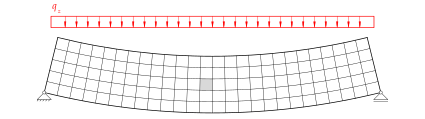
\includegraphics{index_files/mediabag/../images/Kontinua_system.pdf}

}

\caption{\label{fig-system_reine_biegung_system}Statisches System mit
finiten Elementen}

\end{figure}

Die Schnittkräfte am differentiellen Element folgen zu:

\begin{figure}[H]

{\centering 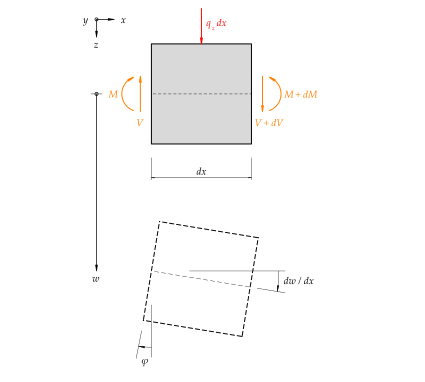
\includegraphics{index_files/mediabag/../images/Kontinua_element.pdf}

}

\caption{\label{fig-system_reine_biegung_element}Differentielles Element
des reinen Beigebalkens}

\end{figure}

Aus Gleichgewicht der vertikalen Kräfte folgt die Beziehung zwischen
Einwirkung und Querkraft:

\[
\downarrow^+\sum F_z = 0 = q_z(x)\cdot dx -V + (V+dV)
\]

\[
q_z(x)\cdot dx = - dV
\]

\begin{equation}\protect\hypertarget{eq-dgl_v_x}{}{
q_z(x) = \frac{dV}{dx} = -V(x)'     
}\label{eq-dgl_v_x}\end{equation}

Aus dem Gleichgewicht der Momente kann die Beziehung zwischen Einwirkung
und Momente ermittelt werden:

\[
\sum^{\curvearrowleft+} M_y = 0 = (M+dM) - M - V \cdot dx + q_z(x)\cdot dx \cdot dx/2
\]

\[
0 = dM - V \cdot dx - \frac{dV}{dx}\cdot dx^2/2
\] \[
0 = \frac{dM}{dx} - V -dV/2
\] \[
V+dV/2 = \frac{dM}{dx} 
\] \begin{equation}\protect\hypertarget{eq-dgl_M_y}{}{
q_z(x) = -V(x)'= -\frac{dM}{dx^2} 
}\label{eq-dgl_M_y}\end{equation}

Die Herleitung etwas abgekürzt ist aus den Stoffgleichungen die
Beziehung zwischen Biegemoment und Krümmung bekannt. Diese sind durch
die Biegesteifigkeit \(EI\) gekoppelt.

\begin{equation}\protect\hypertarget{eq-momentenkruxfcmmung}{}{
\frac{M}{EI} = \chi
}\label{eq-momentenkrümmung}\end{equation}

Aus der verformten Lage lässt sich die Verdrehung des Elements
bestimmen. Die Krümmung beschreibt die Änderung der Verdrehungung.

\begin{equation}\protect\hypertarget{eq-krummung}{}{
\chi = \varphi(x)'
}\label{eq-krummung}\end{equation}

Abschliessend entspricht die Verdrehung der Änderung der Deformation.

\[
-\varphi = \frac{dw}{dx}
\]

Daraus folgt die Beziehung zwischen Biegemoment und Deformation:

\[
M = -EIw(x)''
\]

Und abschliessend die Beziehung zwischen Einwirkung und Deformation:
\begin{equation}\protect\hypertarget{eq-dgl_reine_biegung}{}{
q(x) = EIw(x)''''
}\label{eq-dgl_reine_biegung}\end{equation}

\hypertarget{anwendungen-und-grenzen}{%
\subsection{Anwendungen und Grenzen}\label{anwendungen-und-grenzen}}

Das angewendete Modell berücksichtigt keine Schubverformungen. Da in der
Praxis übliche Stahlbetonbauteile eine signifikant grössere
Schubsteifigkeit, als Biegesteifigkeit besitzen, liefert das Modell
zuverlässige Resultate.

\hypertarget{mohrsche-analogie}{%
\section{Mohrsche Analogie}\label{mohrsche-analogie}}

\hypertarget{aufbau-1}{%
\subsection{Aufbau}\label{aufbau-1}}

Aus den Beziehungen für reine Biegeträger, detailliert beschrieben in
Kapitel~\ref{sec-kontinua}, können folgende Abhängigkeiten definiert
werden:

\[
\frac{d^2M}{dx^2} = M'' = -q_z
\]

\[
\frac{d^2w}{dx^2} = w'' = -\frac{M}{EI}
\]

Erkennbar ist die Analogie der beiden Gleichungen. Aus der Einwirkung
lässt sich der Verlauf der Biegemomente bestimmen. Wird nun auf ein
analoges System der Verlauf der Biegemomente als Einwirkung angesetzt,
so lässt sich mit dem gleichen Berechnungsvorgehen die Deformation
bestimmen. Lediglich den Randbedingungen ist Beachtung zu schenken,
welche mit entsprechenden Lagerungsbedingungen im analogen System
berücksichtigt werden.

\begin{figure}[H]

{\centering 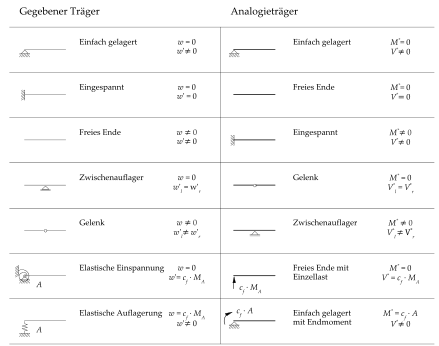
\includegraphics{../images/analogietrager.png}

}

\caption{\label{fig-randbedingungen_analogiesysteme}Lagerugnsbedingungen
für Analogiesysteme}

\end{figure}

\hypertarget{zuggurtmodell}{%
\section{Zuggurtmodell}\label{zuggurtmodell}}

\hypertarget{aufbau-2}{%
\subsection{Aufbau}\label{aufbau-2}}

\bookmarksetup{startatroot}

\hypertarget{zuggurtmodell-1}{%
\chapter{Zuggurtmodell}\label{zuggurtmodell-1}}

\hypertarget{verbundschubspannungs-schlupfbeziehung}{%
\section{Verbundschubspannungs-Schlupfbeziehung}\label{verbundschubspannungs-schlupfbeziehung}}

Die Verbundschuspannungs-Schlupfbeziehung wird in
{[}\protect\hyperlink{ref-Spathelf2022}{2}{]} foglendermassen
postuliert: Es wird hier auf die Stahlspannung sich bezogen, nicht auf
den Schlupf

\begin{equation}\tau_{b}{\left(\sigma_{s} \right)} = \begin{cases} 0 & \text{for}\: \sigma_{s} \leq 0 \\0.6 f_{cc}^{\frac{2}{3}} & \text{for}\: f_{sy} \geq \sigma_{s} \\0.3 f_{cc}^{\frac{2}{3}} & \text{otherwise} \end{cases}\end{equation}

\begin{figure}[H]

{\centering \includegraphics{index_files/mediabag/05_Zuggurtmodell_files/figure-pdf/fig-zg-verbundschubbez-output-1.pdf}

}

\caption{\label{fig-zg-verbundschubbez}Verbundschubspannung als Funktion
der Betonstahlspannung}

\end{figure}

\bookmarksetup{startatroot}

\hypertarget{deformationsberechnung-an-dreipunktbiegeversuch}{%
\chapter{Deformationsberechnung an
Dreipunktbiegeversuch}\label{deformationsberechnung-an-dreipunktbiegeversuch}}

\hypertarget{versuchsbeschrieb}{%
\section{Versuchsbeschrieb}\label{versuchsbeschrieb}}

Gewählt wird aus {[}\protect\hyperlink{ref-Jaeger2006}{3}{]} der
Versuch:

\hypertarget{baustoffeigenschaften}{%
\section{Baustoffeigenschaften}\label{baustoffeigenschaften}}

Aus den Prüfkörper ermittelten Baustoffeigenschaften sind an das Bauteil
anzupassen:

\hypertarget{beton}{%
\subsection{Beton}\label{beton}}

Druckfestigkeit gemäss {[}\protect\hyperlink{ref-Jaeger2014}{4}{]}:

\begin{equation}f_{c} = 2.7 f_{cc}^{\frac{2}{3}}\end{equation}

\begin{equation}f_{c} = \frac{40.827 \text{N}}{\text{mm}^{2}}\end{equation}

Zugfestigkeit nach {[}\protect\hyperlink{ref-Jaeger2013}{5}{]}:

\begin{equation}f_{ct} = 0.3 f_{cc}^{\frac{2}{3}}\end{equation}

\begin{equation}f_{ct} = \frac{4.54 \text{N}}{\text{mm}^{2}}\end{equation}

Elastizitätsmodul nach {[}\protect\hyperlink{ref-Jaeger2013}{5}{]}:

\begin{equation}E_{c} = 10000 \sqrt[3]{f_{cc}}\end{equation}

\begin{equation}E_{c} = \frac{38886.0 \text{N}}{\text{mm}^{2}}\end{equation}

\hypertarget{zustandslinien-fuxfcr-biegetruxe4ger}{%
\section{Zustandslinien für
Biegeträger}\label{zustandslinien-fuxfcr-biegetruxe4ger}}

Nach {[}\protect\hyperlink{ref-Marti}{1}{]} Kapitel 18.4:

Es wird in diesem Kapitel keine Herleitung der Beziehung zwischen
Einwirkung und der Deformation dargestellt. Der Fokus liegt auf der
praktischen Anwendung.

\begin{figure}[H]

{\centering 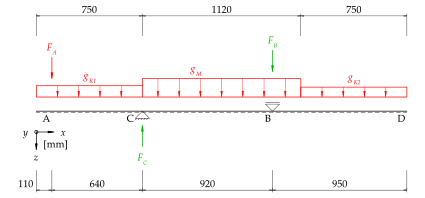
\includegraphics{index_files/mediabag/../images/System_anordnung_2.pdf}

}

\caption{\label{fig-system_2}Statisches System der Versuchsanordnung}

\end{figure}

Das Eigengewicht wird vernachlässigt aus folgenden Gründen:

\begin{itemize}
\tightlist
\item
  Die Punktlast \(F_A\) ist massgebend am Biegemomentenverlauf
  beteiligt.
\item
  Die Deformationen im Versuchsbericht aus
  {[}\protect\hyperlink{ref-Jaeger2006}{3}{]} sind nach dem Einbau des
  Trägers gemessen worden. Folglich wurde die Deformation des
  Eigengewichts nicht aufgezeichnet.
\end{itemize}

\begin{equation}\protect\hypertarget{eq-eigengewicht}{}{
g_M, g_{k1}, g_{k2} = 0
}\label{eq-eigengewicht}\end{equation}

Unter Berücksichtigung der Auflagerbreiten folgt das System in
Abbildung~\ref{fig-system_2_lager}

\begin{figure}[H]

{\centering 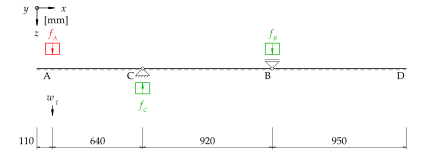
\includegraphics{index_files/mediabag/../images/System_anordnung_2_lagerbreite.pdf}

}

\caption{\label{fig-system_2_lager}Angepasstes statisches System der
Versuchsanordnung}

\end{figure}

Folgende Parameter werden für die Berechnung verwendet:

\begin{longtable}[]{@{}
  >{\raggedright\arraybackslash}p{(\columnwidth - 2\tabcolsep) * \real{0.5000}}
  >{\raggedright\arraybackslash}p{(\columnwidth - 2\tabcolsep) * \real{0.5000}}@{}}
\toprule\noalign{}
\endhead
\bottomrule\noalign{}
\endlastfoot
\(a_{1} = 0.11 \, \text{m}\) & \(a_{2} = 0.64 \, \text{m}\) \\
\(a_{3} = 0.92 \, \text{m}\) & \(a_{4} = 0.95 \, \text{m}\) \\
\(b = 800.0 \, \text{mm}\) & \(b_{Auflager} = 100 \, \text{mm}\) \\
\(h = 200.0 \, \text{mm}\) & \\
\end{longtable}

\hypertarget{auflagerkruxe4fte}{%
\subsection{Auflagerkräfte}\label{auflagerkruxe4fte}}

Durch Gleichgewicht der Momente um Punkt C und B lassen sich die
Auflagerkräfte bestimmen:

Die Balkenlänge bestimmt sich zu:

\begin{equation}l_{tot} = a_{1} + a_{2} + a_{3} + a_{4}\end{equation}

\begin{equation}l_{tot} = 2.62 \text{m}\end{equation}

Durch Gleichgewicht um die Auflagerpunkte folgt:

\begin{equation}0 = F_{A} a_{2} - F_{B} a_{3}\end{equation}

\begin{equation}0 = F_{A} \left(a_{2} + a_{3}\right) - F_{C} a_{3}\end{equation}

Daraus folgen die Reaktionskräfte:

\begin{equation}F_{B} = \frac{F_{A} a_{2}}{a_{3}}\end{equation}

\begin{equation}F_{C} = \frac{F_{A} a_{2} + F_{A} a_{3}}{a_{3}}\end{equation}

Um die Auflagerbreite zu berücksichtigen folgen die Kräfte zu:

\begin{equation}f_{B} = \frac{F_{A} a_{2}}{a_{3} b_{Auflager}}\end{equation}

\begin{equation}f_{C} = \frac{F_{A} a_{2} + F_{A} a_{3}}{a_{3} b_{Auflager}}\end{equation}

\begin{equation}f_{A} = \frac{F_{A}}{b_{Auflager}}\end{equation}

\hypertarget{zustandslinien}{%
\subsection{Zustandslinien}\label{zustandslinien}}

Anhand der Differentialgleichung für Biegeträger können die
Zustandslinien bestimmt werden:

\begin{equation}q{\left(x \right)} = - EI^{I} \frac{d^{4}}{d x^{4}} w\end{equation}

\hypertarget{vollstuxe4ndig-ungerissen}{%
\subsubsection{Vollständig ungerissen}\label{vollstuxe4ndig-ungerissen}}

Die Biegesteifigkeit des ungerissenen Querschnitts folgt zu:

\begin{equation}EI = \frac{E_{c} b h^{3}}{12}\end{equation}

\begin{align}EI = 2.07 \cdot 10^{13} \, \mathrm{Nmm^2} \end{align}

Der Verlauf der Einwirkungen ist der folgende. Die positive Stabseite
ist strichliert dargestellt. Folglich sind Einwirkungen nach ``unten''
positiv definiert.

\begin{figure}[H]

{\centering 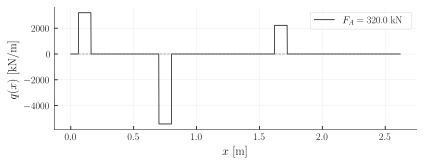
\includegraphics{index_files/mediabag/06_Versuch_2_A3_Jaeger_files/figure-pdf/fig-q_x-output-1.pdf}

}

\caption{\label{fig-q_x}Verlauf der Einwirkungen und Reaktionskräften}

\end{figure}

Durch Integration der Einwirkung resultiert der Querkraftverlauf. Die
Integrationskonstante ist hier null.

\[
V(x) = -\int q(x) + c_1
\]

Dabei kann mit der Randbedingun \(V(0) = 0\) die Integrationskonstante
ermittelt werden.

\begin{figure}[H]

{\centering 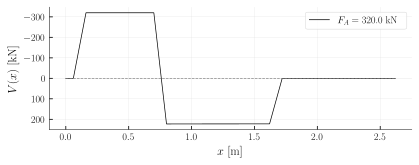
\includegraphics{index_files/mediabag/06_Versuch_2_A3_Jaeger_files/figure-pdf/fig-v_x-output-1.pdf}

}

\caption{\label{fig-v_x}Verlauf der Querkräfte}

\end{figure}

Der Verlauf der Biegemoment lässt sich durch Integration der Querkräfte
bestimmen:

\[
M(x) = \int V(x) + c_2
\]

Dabei kann mit der Randbedingun \(M(0) = 0\) die Integrationskonstante
ermittelt werden.

\begin{figure}[H]

{\centering 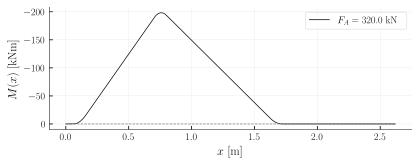
\includegraphics{index_files/mediabag/06_Versuch_2_A3_Jaeger_files/figure-pdf/fig-m_x-output-1.pdf}

}

\caption{\label{fig-m_x}Verlauf der Biegemomente}

\end{figure}

Die Deformationen entsprechen dem Integrierten Verlauf der Biegemomente,
dividiert durch die Biegesteifigkeit, welche als konstant angesetzt
wird.

\begin{equation}\protect\hypertarget{eq-verdrehung}{}{
\varphi(x) = \frac{1}{EI}\int M(x) + c_3
}\label{eq-verdrehung}\end{equation}

\begin{equation}\protect\hypertarget{eq-verformung}{}{
w(x) = \int \varphi(x) + c_4
}\label{eq-verformung}\end{equation}

Dabei wird mit den Randbedingungen \(w(C) = 0\) und \(w(B) = 0\) die
Integrationskonstanten ermittelt.

\begin{figure}[H]

{\centering \includegraphics{index_files/mediabag/06_Versuch_2_A3_Jaeger_files/figure-pdf/cell-30-output-1.pdf}

}

\end{figure}

Dabei folgt die Deformation \(w_1 = w(0.11)\). Das erhaltene Resultat
entspricht einem vollumfänglich ungerissenen Verhalten.

\begin{equation}w_{1} = 3.28 \text{mm}\end{equation}

\hypertarget{abschuxe4tzung-nach-norm}{%
\section{Abschätzung nach Norm}\label{abschuxe4tzung-nach-norm}}

Nach der bestimmten elastischen Deformation kann die Deformation anhand
des vollständig gerissenen Querschnitts nach SIA262 ermittelt werden.
Ohne Druckbewehrung und Kriecheinflüsse folgt die Gleichung zu :

\begin{equation}\protect\hypertarget{eq-w_1_II_sia}{}{
w_{1II,SIA} = \frac{0.75}{10\rho^{0.7}}(\frac{h}{d})^3 w_1
}\label{eq-w_1_II_sia}\end{equation}

Dabei entspricht der geometrische Bewehrugnsgehalt:

\begin{equation}\rho = \frac{A_{s}}{b d}\end{equation}

Die Querschnittsfläche der Stäbe:

\begin{equation}A_{s} = 2 b \frac{\pi \oslash_{s}^{2}}{4 s_{x}}\end{equation}

\begin{equation}A_{s} = 2262.0 \text{mm}^{2}\end{equation}

Die statische Höhe:

\begin{equation}d = - \frac{3 \oslash_{s}}{2} - c_{nom} + h\end{equation}

\begin{equation}d = 162.0 \text{mm}\end{equation}

Die Deformation entspricht abschliessend:

\begin{equation}w_{1 II,SIA} = 15.7 \text{mm}\end{equation}

\hypertarget{mohrsche-analogie-1}{%
\section{Mohr'sche Analogie}\label{mohrsche-analogie-1}}

Die Mohr'sche Analogie basiert auf der selben Modellierung wie in
\ldots{} beschrieben. Durch die Analogie der folgenden zwei
Differentialgleichungen, folgt eine zuverlässige und handhabbare Methode
um Deformationen an einem reinen Biegeträger zu bestimmen.

\[
\frac{d^2M}{dx^2} = M'' = -q_z
\]

\[
\frac{d^2w}{dx^2} = w'' = -\frac{M}{EI}
\]

Wird folglich die Zustandslinie der Biegemomente als Einwirkung auf das
System angesetzt, so entspricht die Biegemomentenlinie dieses System der
Verformungslinie. Lediglich die Randbedingungen sind mit entsprechender
Anpassung der Lagerung des Systems zu berücksichtigen.

Wird nun der bereits bestimmte Momentenverlauf als Einwirkung angesetzt
folgt:

\begin{figure}[H]

{\centering 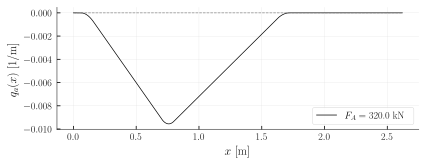
\includegraphics{index_files/mediabag/06_Versuch_2_A3_Jaeger_files/figure-pdf/fig-q_x_mohr-output-1.pdf}

}

\caption{\label{fig-q_x_mohr}Verlauf der Einwirkungen auf das analoge
System}

\end{figure}

Die maximale Biegeverformung tritt beim Stabanfang auf. Da wir mit der
Analogie die Deformation aus den Biegemomenten bestimmen, muss das
Biegemoment bei Stabanfang maximal sein. Dies bedingt eine eine
Einspannung an den freien Enden. Sowie sind bei den ursprünglichen
Auflagern Gelenke einzuführen.

\begin{figure}[H]

{\centering 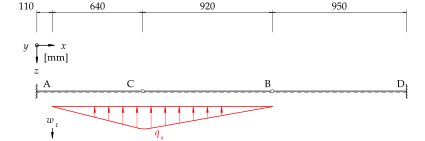
\includegraphics{index_files/mediabag/../images/System_analog.pdf}

}

\caption{\label{fig-system_analog}Analoges System}

\end{figure}

\begin{figure}[H]

{\centering 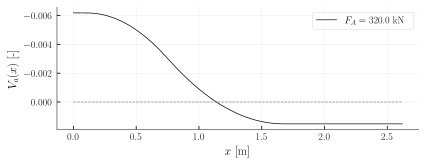
\includegraphics{index_files/mediabag/06_Versuch_2_A3_Jaeger_files/figure-pdf/fig-v_x_mohr-output-1.pdf}

}

\caption{\label{fig-v_x_mohr}Verlauf der Querkräfte für das
Analogiesystem}

\end{figure}

\begin{figure}[H]

{\centering 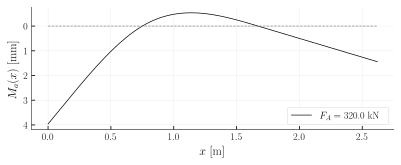
\includegraphics{index_files/mediabag/06_Versuch_2_A3_Jaeger_files/figure-pdf/fig-m_x_mohr-output-1.pdf}

}

\caption{\label{fig-m_x_mohr}Verlauf der Biegemomente für das
Analogiesystem}

\end{figure}

\hypertarget{numerische-integration-der-kruxfcmmung}{%
\section{Numerische Integration der
Krümmung}\label{numerische-integration-der-kruxfcmmung}}

\hypertarget{einfuxfchrung}{%
\subsection{Einführung}\label{einfuxfchrung}}

Ziel ist die Deformationen des Versuchs A3 in der Versuchsanordnung 2
aus {[}\protect\hyperlink{ref-Jaeger2006}{3}{]} nachzurechnen.

\hypertarget{momenten-kruxfcmmungsdiagramm}{%
\subsection{Momenten-Krümmungsdiagramm}\label{momenten-kruxfcmmungsdiagramm}}

Das Momenten-Krümmungsdiagramm ist geeignet zur Beschreibung des
Tragverhaltens von überwiegend auf Biegung beanspruchte Stabtragwerke.
Zur rechnerischen Ermittlung gelten folgende Annahmen, wie in
{[}\protect\hyperlink{ref-Spathelf2022}{2}{]} beschrieben:

\begin{itemize}
\tightlist
\item
  Eben- und senkrechtbleiben der Querschnitte
\item
  Die Betonzugfestigkeit \(f_{ct}\) wird, für Zustände nach dem
  Überschreiten von \(f_{ct}\), vernachlässigt
\item
  Linear elastisches Verhalten von Stahl und Beton für die Spannungs-
  und Verformungsberechnung
\item
  Die Bewehrung überträgt Zug- und Druckkräfte ausschliesslich in
  Stabrichtung
\end{itemize}

\hypertarget{anwendung-auf-versuchsbeispiel}{%
\subsubsection{Anwendung auf
Versuchsbeispiel}\label{anwendung-auf-versuchsbeispiel}}

Folgend wird ein Momentenkrümmungsdiagramm für den Querschnitt aus dem
beschriebenen Versuch berechnet. Die vorhandene Querkraftbewehrung ist
nicht dargestellt in Abbildung~\ref{fig-qs_a3}.

\begin{figure}[H]

{\centering 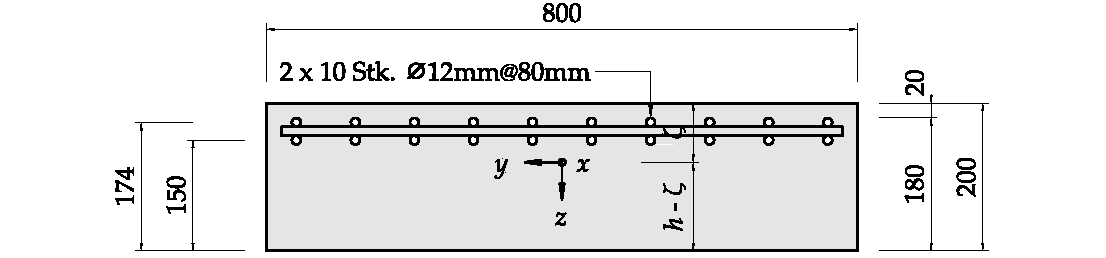
\includegraphics{index_files/mediabag/../images/QS_Versuch_A3.pdf}

}

\caption{\label{fig-qs_a3}Querschnitt des Versuchs A3 zur Bestimmung des
Momenten-Krümmungdiagramms}

\end{figure}

Vereinfacht wird der Querschnitt folgender massen:

\begin{figure}[H]

{\centering 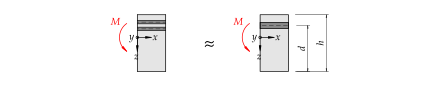
\includegraphics{index_files/mediabag/../images/QS_analyse_1.pdf}

}

\caption{Vereinfachung der Bewehrungsführung}

\end{figure}

\hypertarget{verwendete-parameter}{%
\paragraph{Verwendete Parameter}\label{verwendete-parameter}}

\begin{longtable}[]{@{}
  >{\raggedright\arraybackslash}p{(\columnwidth - 2\tabcolsep) * \real{0.5000}}
  >{\raggedright\arraybackslash}p{(\columnwidth - 2\tabcolsep) * \real{0.5000}}@{}}
\toprule\noalign{}
\endhead
\bottomrule\noalign{}
\endlastfoot
\(E_{s} = 200000.0 \, \frac{\text{N}}{\text{mm}^{2}}\) &
\(\oslash_{s} = 12.0 \, \text{mm}\) \\
\(c_{nom} = 20.0 \, \text{mm}\) &
\(f_{cc} = 58.8 \, \frac{\text{N}}{\text{mm}^{2}}\) \\
\(f_{su} = 630.3 \, \frac{\text{N}}{\text{mm}^{2}}\) &
\(f_{sy} = 546.0 \, \frac{\text{N}}{\text{mm}^{2}}\) \\
\(s_{x} = 80.0 \, \text{mm}\) & \(\varepsilon_{cu} = 0.0023\) \\
\(\varepsilon_{su} = 0.1117\) & \\
\end{longtable}

\hypertarget{baustoffkennlinien}{%
\paragraph{Baustoffkennlinien}\label{baustoffkennlinien}}

\begin{figure}[H]

{\centering \includegraphics{index_files/mediabag/06_Versuch_2_A3_Jaeger_files/figure-pdf/cell-45-output-1.pdf}

}

\end{figure}

\hypertarget{schwerpunkt-des-querschnitts}{%
\paragraph{Schwerpunkt des
Querschnitts}\label{schwerpunkt-des-querschnitts}}

Durch die Bestimmung der Wertigkeit \(n\) kann der Querschnitt als
homogener Betonquerschnitt zur Bestimmung des Schwerpunkts behandelt
werden.

\begin{equation}n = \frac{E_{s}}{E_{c}}\end{equation}

\begin{equation}n = 5.14\end{equation}

Die Querschnittsfläche der Bewehrung:

\begin{equation}A_{s} = 2 b \frac{\pi \oslash_{s}^{2}}{4 s_{x}}\end{equation}

\begin{equation}A_{s} = 2262.0 \text{mm}^{2}\end{equation}

Die Betonquerschnittsfläche:

\begin{equation}A_{c} = b h\end{equation}

\begin{equation}A_{c} = 160000.0 \text{mm}^{2}\end{equation}

Die ideelle Querschnittsfläche resultiert zu:

\begin{equation}A_{i} = A_{c} + A_{s} \left(n - 1\right)\end{equation}

\begin{equation}A_{i} = 169372.0 \text{mm}^{2}\end{equation}

\begin{equation}\zeta_{c} = \frac{\frac{A_{c} h}{2} + A_{s} \left(1.5 \oslash_{s} + c_{nom}\right) \left(n - 1\right)}{A_{i}}\end{equation}

\begin{equation}\zeta_{c} = 96.6 \text{mm}\end{equation}

\hypertarget{fluxe4chentruxe4gheitsmoment}{%
\paragraph{Flächenträgheitsmoment}\label{fluxe4chentruxe4gheitsmoment}}

Das Flächenträgheitsmoment wird ebenfalls am ideellen Querschnitt
bestimmt. Die Eigenträgheitsmomente der Kreisquerschnitte der Bewehrung
sind nicht berücksichtigt, lediglich der Steiner-Anteil fliesst in die
Berechnung ein:

\begin{equation}I^{I} = A_{s} \left(n - 1\right) \left(\frac{3 \oslash_{s}}{2} + c_{nom} - \zeta_{c}\right)^{2} + \frac{b h^{3}}{12} + b h \left(\frac{h}{2} - \zeta_{c}\right)^{2}\end{equation}

\begin{equation}I^{I} = 5.67 \cdot 10^{8} \text{mm}^{4}\end{equation}

\hypertarget{ungerissen---zustand-1}{%
\paragraph{Ungerissen - Zustand 1}\label{ungerissen---zustand-1}}

Der Querschnitt verbleibt elastisch. Folglich kann das
Flächenträgheitsmoment mit \(E_c\) multipliziert werden und es
resultiert die ungerissene Biegesteifigkeit:

\begin{equation}EI^{I} = E_{c} I^{I}\end{equation}

\begin{align}EI^{I} = 2.206 \cdot 10^{13} \, \mathrm{Nmm^2} \end{align}

\hypertarget{rissmoment}{%
\subparagraph{Rissmoment}\label{rissmoment}}

Durch die Ermittlung des Rissmoments kann die Krümmung vor dem Reissen
des Betons ermittelt werden. Die Betonzugkraft wird nicht
berücksichtigt.

\begin{figure}[H]

{\centering 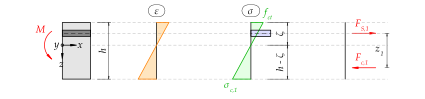
\includegraphics{index_files/mediabag/../images/QS_analyse_2.pdf}

}

\caption{\label{fig-qs2}Querschnittsanalyse vor dem Reissen des Betons}

\end{figure}

Die Druckspannung bestimmt sich zu:

\begin{equation}\sigma_{c inf,1} = \frac{f_{ct} \left(h - \zeta_{c}\right)}{\zeta_{c}}\end{equation}

\begin{equation}\sigma_{c inf,1} = \frac{4.86 \text{N}}{\text{mm}^{2}}\end{equation}

Der Hebelarm der inneren Kräfte:

\begin{equation}z_{1} = - 1.5 \oslash_{s} - c_{nom} + \frac{2 h}{3} + \frac{\zeta_{c}}{3}\end{equation}

\begin{equation}z_{1} = 128.0 \text{mm}\end{equation}

Die Betondruckkraft:

\begin{equation}F_{c,1} = \frac{b \sigma_{c inf,1} \left(h - \zeta_{c}\right)}{2}\end{equation}

\begin{equation}F_{c,1} = 2.01 \cdot 10^{5} \text{N}\end{equation}

Und schliesslich das Rissmoment:

\begin{equation}M_{r} = F_{c,1} z_{1}\end{equation}

\begin{align}M_{r} = 2.56 \cdot 10^{7} \, \mathrm{Nmm} \end{align}

Aus dem Rissmoment folgt die Krümmung beim Reissen:

\begin{equation}\chi_{r} = \frac{M_{r}}{EI^{I}}\end{equation}

\begin{equation}\chi_{r} = \frac{0.00116}{\text{m}}\end{equation}

\hypertarget{gerissen-elastisch---zustand-2}{%
\paragraph{Gerissen Elastisch - Zustand
2}\label{gerissen-elastisch---zustand-2}}

Der Querschnitt nach dem Reissen ist in Abbildung~\ref{fig-qs3}
dargestellt. Der Betonstahl hat die Fliessgrenze noch nicht erreicht.
Der Beton die Druckfestigkeit ebenfalls nicht.

\begin{figure}[H]

{\centering 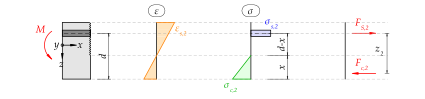
\includegraphics{index_files/mediabag/../images/QS_analyse_3.pdf}

}

\caption{\label{fig-qs3}Querschnittsanalyse nach dem Reissen des Betons}

\end{figure}

Dabei beträgt die statische Höhe:

\begin{equation}d = - \frac{3 \oslash_{s}}{2} - c_{nom} + h\end{equation}

\begin{equation}d = 162.0 \text{mm}\end{equation}

Nachfolgend werden bekannte Beziehungen dargestellt. Mittels
Gleichgewicht der Kräfte lässt sich die Betondruckzonenhöhe und folglich
die gerissene Biegesteifigkeit herleiten.

Die Betonstahlzugkraft beträgt:

\begin{equation}F_{z,2} = A_{s} \sigma_{s,2}\end{equation}

Die Betonstahlspannung für linear elastisches Verhalten:

\begin{equation}\sigma_{s,2} = E_{s} \varepsilon_{s,2}\end{equation}

Die Betondruckkraft anhand des dreieckigen Verlaufs in
Abbildung~\ref{fig-qs3}:

\begin{equation}F_{c,2} = \frac{b \sigma_{c inf,2} x_{2}}{2}\end{equation}

Die Betonspannung ebenfalls bestimmt durch ein linear elastisches
Verhalten:

\begin{equation}\sigma_{c inf,2} = E_{c} \varepsilon_{c,2}\end{equation}

Die Betondehnung anhand des Dehnungsverlaufs in Abbildung~\ref{fig-qs3}:

\begin{equation}\varepsilon_{c,2} = \frac{\varepsilon_{s,2} x_{2}}{d - x_{2}}\end{equation}

Abschliessend sind die Kräfte ins Gleichgewicht zu setzen:

\begin{equation}F_{c,2} = F_{z,2}\end{equation}

Einsetzen der bestimmten Gleichungen in die Gleichgewichtsbeziehung:

\begin{equation}n = \frac{E_{s}}{E_{c}}\end{equation}

\begin{equation}\rho = \frac{A_{s}}{b d}\end{equation}

Dabei wird mit \(n\) und \(\rho\) substituiert um die Gleichung zu
vereinfachen.

\begin{equation}E_{s} b d \rho \varepsilon_{s,2} = \frac{E_{s} b \varepsilon_{s,2} x_{2}^{2}}{2 n \left(d - x_{2}\right)}\end{equation}

Dies ist nach \(x\) aufzulösen:

\begin{equation}x_{2} = d \left(- n \rho + \sqrt{n \rho \left(n \rho + 2\right)}\right)\end{equation}

\begin{equation}x_{2} = 55.6 \text{mm}\end{equation}

Zur Bestimmung der Krümmung ist die Betonstahldehnung erforderlich.
Diese bedingt ein einwirkendes Moment. Dazu wird das bereits bekannte
Rissmoment angesetzt.

\begin{equation}M_{2} = F_{z,2} \left(d - \frac{x_{2}}{3}\right)\end{equation}

\begin{equation}M_{2} = M_{r}\end{equation}

\begin{equation}M_{r} = A_{s} E_{s} \varepsilon_{s,2} \left(d - \frac{x_{2}}{3}\right)\end{equation}

Daraus resultiert die Betonstahldehnung:

\begin{equation}\varepsilon_{s,2} = 0.000395\end{equation}

Die Krümmung kann anhand des Dehnungsverlaufs in Abbildung~\ref{fig-qs3}
bestimmt werden:

\begin{equation}\chi^{II} = \frac{\varepsilon_{s,2}}{d - x_{2}}\end{equation}

\begin{equation}\chi^{II} = \frac{0.00371}{\text{m}}\end{equation}

Abschliessend folgt die gerissene Biegesteifigkeit zu:

\begin{equation}EI^{II} = \frac{M_{2}}{\chi^{II}}\end{equation}

\begin{align}EI^{II} = 6.9 \cdot 10^{12} \, \mathrm{Nmm^2} \end{align}

\hypertarget{fliessen-der-bewehrung---zustand-3}{%
\paragraph{Fliessen der Bewehrung - Zustand
3}\label{fliessen-der-bewehrung---zustand-3}}

Die Biegesteifigkeit \(EI^{II}\) gilt bis die Bewehrung fliesst oder der
Beton beginnt zu plastifizieren.

\begin{figure}[H]

{\centering 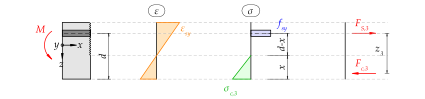
\includegraphics{index_files/mediabag/../images/QS_analyse_4.pdf}

}

\caption{\label{fig-qs4}Querschnittsanalyse für reine Biegung beim
Fliessen der Bewehrung}

\end{figure}

Dazu gilt es zuerst Gleichgewicht der Kräfte zu formulieren:

\begin{equation}\sigma_{c inf,3} = \frac{E_{c} f_{sy} x_{3}}{E_{s} \left(d - x_{3}\right)}\end{equation}

\begin{equation}A_{s} f_{sy} = \frac{b \sigma_{c inf,3} x_{3}}{2}\end{equation}

Aufgelöst nach der Druckzonenhöhe:

\begin{equation}x_{3} = \frac{- A_{s} E_{s} + \sqrt{A_{s} E_{s} \left(A_{s} E_{s} + 2 E_{c} b d\right)}}{E_{c} b}\end{equation}

\begin{equation}x_{3} = 55.6 \text{mm}\end{equation}

Daraus lässt sich das Fliessmoment bestimmen, welches den Endpunkt im
Momenten-Krümmungsdiagramm für den Zustand 2 definiert:

\begin{equation}M_{y} = A_{s} f_{sy} \left(d - \frac{x_{3}}{3}\right)\end{equation}

\begin{equation}M_{y} = 1.77 \cdot 10^{8} \text{mm} \text{N}\end{equation}

Die Fliessdehnung des Betonstahls entspricht:

\begin{equation}\varepsilon_{sy} = 0.00273\end{equation}

Abschliessend die Krümmung für den Endpunkt des Zustands 2:

\begin{equation}\chi_{y} = \frac{\varepsilon_{sy}}{d - x_{3}}\end{equation}

\begin{equation}\chi_{y} = \frac{2.57 \cdot 10^{-5}}{\text{mm}}\end{equation}

\hypertarget{maximaler-biegewiderstand---zustand-4}{%
\paragraph{Maximaler Biegewiderstand - Zustand
4}\label{maximaler-biegewiderstand---zustand-4}}

Abschliessen kann der maximale Biegewiderstand durch die plastifizierung
der Betondruckzone bestimmt werden. Dem Stahl wird die statische
Zugfestigkeit vorausgesetzt, dies berücksichtigt eine Verfestigung.
Sowie gilt es zu kontrollieren, ob die Betonstahldehnung unterhalb der
Bruchdehnung liegt.

\begin{figure}[H]

{\centering 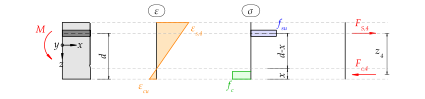
\includegraphics{index_files/mediabag/../images/QS_analyse_5.pdf}

}

\caption{\label{fig-qs5}Querschnittsanalyse für reine Biegung beim
Fliessen der Bewehrung und plastifizierter Betondruckzone}

\end{figure}

Vereinfacht werden die Spannungen in der Druckzone konstant verteilt
betrachtet. Dazu wird die Druckzonenhöhe abgemindert um Faktor 0.85.

Das Gleichgewicht der Kräfte führt zu:

\begin{equation}A_{s} f_{su} = 0.85 b f_{c} x_{4}\end{equation}

Die Druckzonenhöhe folgt zu:

\begin{equation}x_{4} = 51.4 \text{mm}\end{equation}

\begin{equation}M_{R} = A_{s} f_{su} \left(d - 0.425 x_{4}\right)\end{equation}

\begin{align}M_{R} = 199848.0 \, \mathrm{Nm} \end{align}

Die Krümmung lässt sich anhand der Betonstauchung ermitteln:

\begin{equation}\chi_{u} = \frac{\varepsilon_{cu}}{x_{4}}\end{equation}

\begin{equation}\chi_{u} = \frac{4.48 \cdot 10^{-5}}{\text{mm}}\end{equation}

Die Betonstahldehnung darf die Bruchdehnung nicht überschreiten:

\begin{equation}\varepsilon_{s,4} = \frac{\varepsilon_{cu} \left(d - x_{4}\right)}{x_{4}}\end{equation}

\begin{equation}\varepsilon_{s,4} = 0.00496\end{equation}

Die Bruchdehnung des Stahls wird nicht überschritten. Der Querschnitt
versagt im Druckbereich:

\begin{equation}\varepsilon_{su} = 0.1117\end{equation}

Die Biegesteifigkeit im Bereich 3 beträgt:

\begin{equation}EI^{III} = \frac{M_{R}}{\chi_{u}}\end{equation}

\begin{equation}EI^{III} = 4.46 \cdot 10^{6} \text{m}^{2} \text{N}\end{equation}

Im Bereich drei werden die zwei definierten Punkte \(M_y, \chi_y\) sowie
\(M_R, \chi_u\) verbunden.

\hypertarget{momenten-kruxfcmmungsdiagramm-1}{%
\paragraph{Momenten-Krümmungsdiagramm}\label{momenten-kruxfcmmungsdiagramm-1}}

Abschliessend lässt sich daraus die Beziehung zwischen Moment und
Krümmung darstellen. Der lineare verlauf im ersten Bereich ergibt sich
aus der ungerissenen Biegesteifigkeit. Darauf folgt ein schlagartiger
wechsel der Steifigkeit von \(EI^I\) zu \(EI^{II}\), da der Beton
reisst. Dies führt zum Plateau im unteren Bereich.

\begin{figure}[H]

{\centering 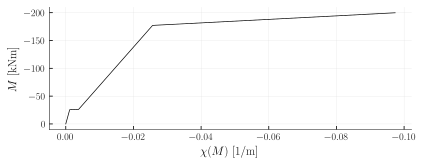
\includegraphics{index_files/mediabag/06_Versuch_2_A3_Jaeger_files/figure-pdf/fig-mchi_diagramm-output-1.pdf}

}

\caption{\label{fig-mchi_diagramm}Momenten-Krümmungsdiagramm händisch
ermittelt, definiert im positiven Bereich}

\end{figure}

\hypertarget{zustandslinien-der-biegemomente}{%
\paragraph{Zustandslinien der
Biegemomente}\label{zustandslinien-der-biegemomente}}

Da die Beziehung zwischen Biegemoment und Krümmung bestimmt ist, kann
ein Krümmungsverlauf über die Stabachse ermittelt werden. Dieser ist
abhängig von der Funktion der Biegemomente zur Stabachse. Die
Zustandslinie der Biegemomente wird anhand des statischen Systems in
Abbildung~\ref{fig-system_2_lager}.

\hypertarget{zustandslinien-der-kruxfcmmung}{%
\paragraph{Zustandslinien der
Krümmung}\label{zustandslinien-der-kruxfcmmung}}

Die Funktion der Biegemomente \(M(x)\) als Eingabe in die Funktion der
Krümmung \(\chi(M)\) resultiert zu folgender Zustandslinie der Krümmung.

\begin{figure}[H]

{\centering 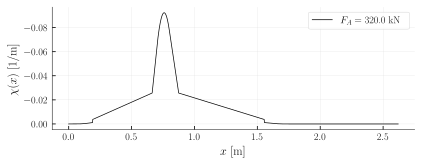
\includegraphics{index_files/mediabag/06_Versuch_2_A3_Jaeger_files/figure-pdf/fig-chi_x_diagramm-output-1.pdf}

}

\caption{\label{fig-chi_x_diagramm}Krümmungsverlauf für die Laststufe
LS14 entlang der Stabachse}

\end{figure}

\hypertarget{punktuelle-bestimmung-der-deformation}{%
\subsubsection{Punktuelle Bestimmung der
Deformation}\label{punktuelle-bestimmung-der-deformation}}

Unter Anwendung der Arbeitsgleichung kann die Deformation nach
Gleichung~\ref{eq-arbeitsgleichung} bestimmt werden.

\begin{equation}\protect\hypertarget{eq-arbeitsgleichung}{}{
w = \int_0^l \bar{M}(x) \cdot \frac{M(x)}{EI} d_x
}\label{eq-arbeitsgleichung}\end{equation}

Wobei \(\frac{M(x)}{EI} = \chi(x)\) gilt.

Das heisst es gilt die Zustandslinien der Krümmung multipliziert mit der
Zustandslinie der Biegemomente des virtuellen Kräftezustands über die
Stablänge zu integrieren.

\begin{figure}[H]

{\centering \includegraphics{index_files/mediabag/06_Versuch_2_A3_Jaeger_files/figure-pdf/fig-m_y_diagramm_virtuell-output-1.pdf}

}

\caption{\label{fig-m_y_diagramm_virtuell}Biegemomentenverlauf für den
virtuellen Kräftezustand}

\end{figure}

Unter Anwedung der Gleichung~\ref{eq-arbeitsgleichung} folgt die
Deformation bei der Krafteinleitung \(F_A\) zu:

\hypertarget{erweiterung-momenten-kruxfcmmungsdiagramm}{%
\section{Erweiterung
Momenten-Krümmungsdiagramm}\label{erweiterung-momenten-kruxfcmmungsdiagramm}}

\hypertarget{zugversteifung}{%
\subsection{Zugversteifung}\label{zugversteifung}}

Die bisherige Betrachtung beschränkt sich auf einen schlagartigen
Wechsel von ungerissen zu vollständig gerissen. Dabei wird der Bereich
zwischen den Rissen ebenfalls als gerissen angenommen. Mittels der
Zugversteifung wird ein theoretischer Rissabstand ermittelt und zwischen
den Rissen eine versteifte Wirkung zwischen Betonstahl und Beton
angenommen (Verbundwirkung). Dies wird folgend auf das Versuchsbeispiel
angewendet. Berücksichtigt wird dies via dem Ansatz von Marti.

Die Krümmungsdifferenez nach Marti beträgt:

\begin{equation}\Delta\chi{\left(\lambda \right)} = \frac{\lambda}{2} \frac{f_{ct} \left(1 - \rho_{eff}\right)}{E_{s} \rho_{eff} \left(d - x_{2}\right)}\end{equation}

\begin{equation}\rho_{eff} = \frac{1}{- n + 1 + \frac{E_{s} M_{r} \left(d - x_{2}\right)}{EI^{II} f_{ct}}}\end{equation}

\begin{equation}s_{rm} = \frac{\oslash_{s} \lambda \left(1 - \rho_{eff}\right)}{4 \rho_{eff}}\end{equation}

\begin{equation}\sigma_{sr0} = \frac{F_{z,2}}{A_{s}}\end{equation}

\begin{equation}w_{r} = \frac{s_{rm} \left(- \lambda \sigma_{sr0} + 2 \sigma_{sr}\right)}{2 E_{s}}\end{equation}

\begin{equation}\Delta\chi{\left(\lambda \right)} = \frac{0.00131 \lambda}{\text{m}}\end{equation}

\begin{equation}\rho_{eff} = 0.0753\end{equation}

\begin{equation}s_{rm} = 36.8 \lambda \text{mm}\end{equation}

\begin{figure}[H]

{\centering 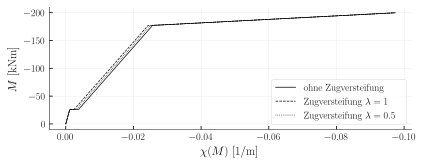
\includegraphics{index_files/mediabag/06_Versuch_2_A3_Jaeger_files/figure-pdf/fig-mchi_diagramm_zugversteifung-output-1.pdf}

}

\caption{\label{fig-mchi_diagramm_zugversteifung}Momenten-Krümmungsdiagramm
mit Zugversteifung ergänzt}

\end{figure}

\begin{figure}[H]

{\centering \includegraphics{index_files/mediabag/06_Versuch_2_A3_Jaeger_files/figure-pdf/fig-chi_x_diagramm_zugversteifung-output-1.pdf}

}

\caption{\label{fig-chi_x_diagramm_zugversteifung}Krümmungsverlauf für
die Laststufe mit Zugversteifung}

\end{figure}

\hypertarget{vergleich-der-ansuxe4tze}{%
\subsection{Vergleich der Ansätze}\label{vergleich-der-ansuxe4tze}}

\begin{figure}[H]

{\centering 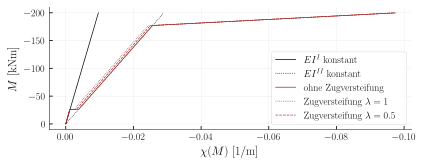
\includegraphics{index_files/mediabag/06_Versuch_2_A3_Jaeger_files/figure-pdf/fig-mchi_diagramm_vergleich-output-1.pdf}

}

\caption{\label{fig-mchi_diagramm_vergleich}Momenten-Krümmungsdiagramm
mit unterschiedlichen Ansätzen}

\end{figure}

\begin{figure}[H]

{\centering \includegraphics{index_files/mediabag/06_Versuch_2_A3_Jaeger_files/figure-pdf/fig-last_verformung-output-1.pdf}

}

\caption{\label{fig-last_verformung}Last-Verformungsdiagramm bei der
Krafteinleitung \(F_A\)}

\end{figure}

\bookmarksetup{startatroot}

\hypertarget{literatur}{%
\chapter*{Literatur}\label{literatur}}
\addcontentsline{toc}{chapter}{Literatur}

\markboth{Literatur}{Literatur}

\hypertarget{refs}{}
\begin{CSLReferences}{0}{0}
\leavevmode\vadjust pre{\hypertarget{ref-Marti}{}}%
\CSLLeftMargin{1. }%
\CSLRightInline{Marti P Baustatik. Wiley-VCH Verlag GmbH}

\leavevmode\vadjust pre{\hypertarget{ref-Spathelf2022}{}}%
\CSLLeftMargin{2. }%
\CSLRightInline{Spathelf C (2022) Skript Teil 2: Gebrauchstauglichkeit.
Betonbau - Ausgewählte Kapitel Hochschule Technik \& Architektur Luzern}

\leavevmode\vadjust pre{\hypertarget{ref-Jaeger2006}{}}%
\CSLLeftMargin{3. }%
\CSLRightInline{Jäger T, Marti P (2006) Versuche zum
{Querkraftwiderstand} und zum {Verformungsvermögen} von
{Stahlbetonplatten}. IBK Bericht 294.
\url{https://doi.org/10.3929/ethz-a-005195576}}

\leavevmode\vadjust pre{\hypertarget{ref-Jaeger2014}{}}%
\CSLLeftMargin{4. }%
\CSLRightInline{Jaeger T (2014) Extended sandwich model for reinforced
concrete slabs: Shear strength with transverse reinforcement.
Engineering Structures 74:218--228.
https://doi.org/\url{https://doi.org/10.1016/j.engstruct.2014.05.025}}

\leavevmode\vadjust pre{\hypertarget{ref-Jaeger2013}{}}%
\CSLLeftMargin{5. }%
\CSLRightInline{Jaeger T (2013) Extended sandwich model for reinforced
concrete slabs: Shear strength without transverse reinforcement.
Engineering Structures 56:1142--1153.
https://doi.org/\url{https://doi.org/10.1016/j.engstruct.2013.06.035}}

\end{CSLReferences}



\end{document}
